\chapter{Cluster Analysis: Basic Concepts and Algorithms}

{\bf Clustering for understanding:} classes, or conceptually meaningful groups of 
objects that share common characteristics, play an important role in how people 
analyze and describe the world. Indeed, human beings are skilled at dividing
objects into groups (clustering) and assigning particular objects to these 
groups (classification).

{\bf Clustering for utility:} In the context of utility, cluster analysis is the
study of techniques for finding the most representative cluster prototypes. 
Some of these techniques are: summarization, compression and finding nearest neighbors.

\clearpage
\section{Overview}
	
	\subsection{What Is Cluster Analysis}

	Cluster analysis groups data objects based only on information found in the 
	data that describes the objects and their relationships. The goal is that the
	objects within a group be similar (or related) to one another and different
	from (or unrelated to) to the objects in other groups. 

	Clustering can also be regarded as a form of classification.
	In contrast, classification in the sense of chapter 4 is {\bf supervised classifiction};
	i.e., new, unlabeled objects are assigned a class label using a model developed
	from objects with known class labels. For this reason, cluster analysis
	is sometimes referred to as {\bf unsupervised classification}.

	The terms {\bf segmentation} and {\bf partitioning} are somtimes used as
	synonyms for clustering.

	\subsection{Different Types of Clusterings}

		An entire collection of clusters is commonly referred to as {\bf clustering}, and
		in this section, we distinguish various types of clusterings: hierarchical (nested)
		vs. partitional (unnested), exclusive vs. overlapping vs. fuzzy, and complete vs. 
		partial. 

		\subsection*{Hierarchical vs. Partitional} 
		A {\bf partitional clustering} is simply a division of the set of data objects into
		non-overlapping subsets (clusters) such that each data object is in exactly one subset.
		If we permit clusters to have subclusters, then we obtain a {\bf hierarchical clustering},
		which is a set of nested clusters that are organized as a tree. Each node (cluster)
		in the tree (expect for the leaf nodes) is the union of its children (subclusters),
		and the root of the tree is the cluster containing all the objects. 

		\subsection*{Exclusive vs. Overlapping vs. Fuzzy}
		When a clustering is {\bf exclusive}, we assign each object to a single cluster.
		In the most general sense, an {\bf overlapping} or {\bf non-exclusive clustering} 
		is used to reflect the fact that an object can simultaneously belong to more than
		one group (class). For instance, a person at a university can be both an enrolled
		student and an employee of the university. 
		In {\bf Fuzzy clustering}, every object belongs to every cluster with a membership
		weight that is between 0 (absolutely doesn't belong) and 1 (absolutely belongs).
		In fuzzy clustering, we often impose the additional constraint that the sum of the
		weights for each object must equal to 1.  

		\subsection*{Complete vs. Partial}
		A {\bf complete clustering} assigns every object to a cluster, wheras a {\bf partial clustering}
		does not. The motivation for a partial clustering is that some objects in a data 
		set may not belong to well-defined groups. Many times objects in the data set may
		represent noise, outliners, or "uninteresting background."

	\clearpage
	\subsection{Different Types of Clusters}

		\begin{itemize}
			\item {\bf Well-seperated:} Figure 7.1a represents well-seperated clusters.
			Each point is closer to all of the points in its cluster than to any point 
			in another cluster.
			\item {\bf Prototype-Based:} Figure 7.1b shows a prototyped-based (center-based)
			clusters. Each point is closer to the center of its cluster than to the center of any
			other cluster. 
			\item {\bf Graph-Based:} If the data is represented as a graph, where the nodes
			are objects annd the links represent connections among objects, then a cluster can be
			defined as a {\bf connected component}; i.e., a group of objects that are connected
			to one another, but that have no connection to objects outside the group. An
			important example of graph-based clusters are {\bf contingency-based clusters}, where
			two objects are connected only if they are within a specified distance of each other. 
			Each point is closer to at least one point in its cluster than to any point in another 
			cluster, Figure 7.1c. 
			\item {\bf Density-Based:} A cluster is a dense region of objects that is surrounded by
			a region of low density. Figure 7.1d shows a density-based cluster.
			\item {\bf Shared-Property (Conceptual Clusters):} We can define a cluster as a set of 
			objects that share some property. Figure 7.1e shows an example of conceptual clusters.
		\end{itemize} 



		\begin{figure}[H]
			\centering
			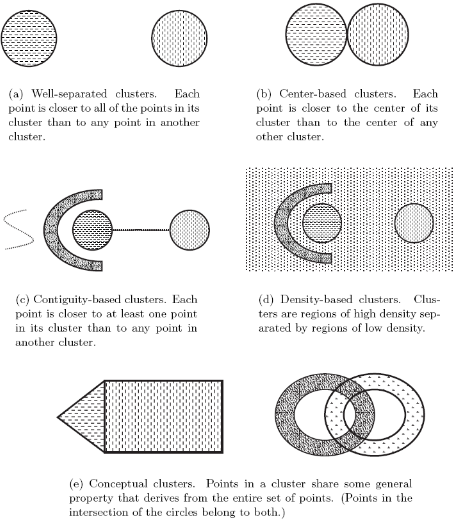
\includegraphics[scale=0.6]{pics/clusters.png}
			\caption{Different types of clusters as illustrated by seys of two-dimensional points}
		\end{figure}

	\clearpage
	\section{K-means}
		This is a prototype-based, partitional clustering technique that attempts to find a
		user-specified number of clusters (K), which are represented by their centroids. 
		K-means defines a prototype in terms of a centroid, which is usually the mean of a 
		group of points. {\bf K-medoid} is almost the same as K-means with centroids, but a centroid
		does not to be an actual data point, while a mendoid does need to be an actual data point.

		{\bf The basic K-means algorithm:} we first choose K initial centroids, where K is a 
		user-specified parameter, namely, the number of clusters desired. Each data point is then
		assigned to the closest centroid, and each collection of ponts assigned to a centroid is a
		cluster. The centroid of each cluster is then updated based on the points assigned to the
		cluster. We repeat the assignment and update steps until no point changes cluster, or 
		equivalently, until the centroids remain the same.

		\begin{figure}[H]
			\centering
			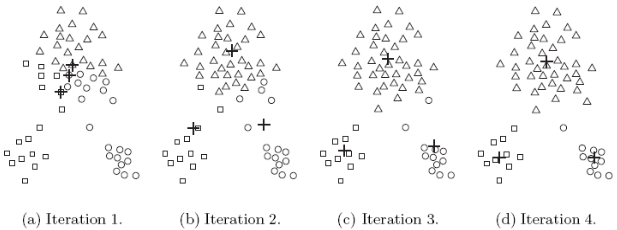
\includegraphics[width=\textwidth]{pics/iterations.png}
			\caption{Using the k-means algorithm to find three clusters in sample data}

		\end{figure} 

		{\bf Assigning Points to the closest centroid:}	To assign a point to the closest centroid, 
		we need a proximity measure that quantifies the notion of "closest" for the specific data
		under consideration. Once we have a specified a proximity measure and an objective function, 
		the centroid that we should choose can often be determined mathematically. 

		{\bf Data in euclidean space:} Consider data whose proximity measure is Euclidean distance.
		For our objective function, which measures the quality of a clustering, we use the 
		{\bf sum of squared error (SSE)}, which is also known as scatter. In other words, we 
		calculate the error of each data point, i.e., its Euclidean distance to the closest centroid,
		and then compute the total sum of the squared errors. 

		\begin{equation}
			SSE = \sum_{i=1}^{K}\sum_{x E C_{i}}^{} dist(c_{i}, x)^{2}
		\end{equation}

		\begin{equation}
			c_{i} = \frac{1}{m_{i}} \sum_{x E C_{i}}^{} x
		\end{equation}

		\clearpage
		{\bf Document Data:} our objective is to maximize the similarity of the documents in a 
		cluster to the cluster centroid; this quantity is known as the {\bf cohesion} of the
		cluster. For this objective it can be shown that the cluster centroid is, as for
		Euclidean data, the mean. The analogous quantity to the total SSE is the total cohesion.

		\begin{equation}
			Total Cohesion = \sum_{i=1}^{K}\sum_{x E C_{i}}^{} cosine(x, c_{i})
		\end{equation}

		{\bf Choosing Initial Centroids:}\\
		\begin{itemize}
			\item Centroids are often choosen randomly
			\item Random otften gives a poor result because the probability of hitting a cluster.
			\item Possible solutions:
				\begin{itemize}
					\item Gjør klyngingen flere ganger og velg det beste (mht. SSE)
					(Sannsynligheten ikke på vår side!) 
					\item Sampling og bruk av hierarkisk klynging for å finne initielle 
					sentroider (Kun for lav verdi av K og små sample)
					\item Velg mer enn K punkt og velg blant disse • Feks. mest mulig separert
					(Gjort på sample for å redusere sjanse for outlier)
					\item Post/pre-prosessering 
					\item Bisecting K-means
				\end{itemize}
		\end{itemize}

		\begin{table}[H]
			\begin{tabular}{| l | l | p{8cm} |}
				\hline
				{\bf Proximity function} & {\bf Centroid} & {\bf Objective function} \\ \hline
				Manhattan ($L_{1}$) & median
				& Minimize sum of the $L_{1}$ distance of an object to its cluster centroid. \\ \hline
				Squared Euclidean ($L_{2}^{2}$) & mean
				& Minimize sum of the squared $L_{2}$ distance of an object to its cluster centroid \\ \hline
				cosine & mean 
				& Maximize sum of the cosine similarity of an object to its cluster centroid. \\ \hline
				Bergman Divergence & mean &
				Minimize sum of the Bergman divergence of an object to its cluster centroid. \\ \hline
			\end{tabular}
			\caption{Commom choices for proximity, centroids, and objective functions}
		\end{table}

		\subsection{K-means: Additional Issues}
			\begin{itemize}
				\item {\bf Handling empty clusters:}
				\item {\bf Outliners:}
				\item {\bf Reducing the SSE with postprocessing}
					\begin{itemize}
						\item Slit a cluster: The cluster with the largest SSE is usually chosen.
						\item Introduce a new cluster centroid: Often the point that is farthest from
						any cluster is chosen, of choose randomly. 
						\item Disperse a cluster: this as accomplished by removing the centroid that
						corresponds to the cluster and reassigning the points to other clusters. 
						Ideally, the cluster that is dispersed should be the one that increase the
						total SSE the least. 
						\item Merge two clusters: The clusters with the closests centroids are 
						typically chosen.
					\end{itemize}
				\item {\bf Updating centroids incrementally:} instead of updating cluster centroids
				after all points have been assigned to a cluster, the centroids can be updated
				incrementall, after each assignment of a point to a cluster. 
			\end{itemize}

		\subsection{Bisecting K-means}

		The bisecting K-means algorithm is a straightforward extension of the basic K-menas algorithm
		that is based on a simple idea: to obtain K clusters, split the set of all points into two
		clusters, select one of these clusters to split, and so on, until K clusters have been 
		produced. 

		\subsection{K-means and Different types of Clusters}

		K-means and its variations have a number of limitations with respect to finding different 
		types of clusters. In particular, K-means have difficulty detecting the "natural" clusters,
		when clusters have different size, different density or non-globular clusters. 

		
	\section{Agglomerative Hierarchical Clustering}
		{\bf Different types of hierarchical clustering:}
		\begin{itemize}
			\item {\bf Agglomerative:} start at the points as individual clusters
			and, at each step, merge the closest pair of clusters.
			\item {\bf Divisive:} Start with one, all-inclusive cluster, and at each
			step, split a cluster until only singelton clusters of individual points
			remain. 
		\end{itemize}

		A hierarchical clustering is often displayed graphically using a tree-like diagram
		called a {\bf dendrogram}, which displays both the cluster-subcluster relationship
		and the order in which the clusters are merged (agglomerative view) or split 
		(divisive view). 

		\begin{figure}[H]
			\centering
			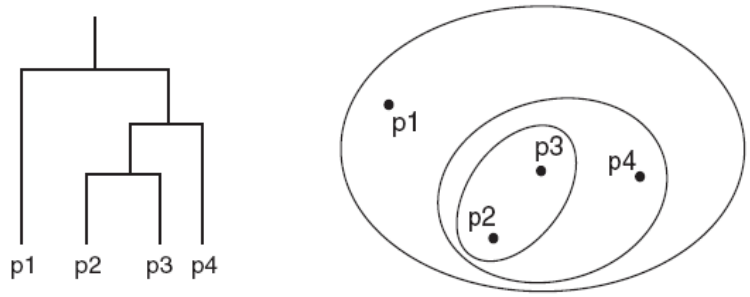
\includegraphics[scale=0.3]{pics/hierarchical.png}
			\caption{Dendrogram and nested cluster diagram}
		\end{figure}

		\clearpage
		{\bf Defining Proximity between Clusters}
		\begin{itemize}
			\item {\bf MIN/single link:} defines cluster proximity as the proximity between the closest
			two points that are in different clusters, or using graph terms, the shortest edge between
			two nodes in different subsets of nodes. 
			\item {\bf MAX/CLIQUE/complete link:} takes the proximity between the farthest two points in different
			clusters to be the cluster proxximity, or using graph terms, the longest edge between 
			two nodes in different subsets of nodes. 
			\item {\bf Group average:} defines cluster proximity to be the average pairwise proximities
			(average length of edges) of all pairs of points from different clusters. 
		\end{itemize}

		\begin{figure}[H]
			\centering
			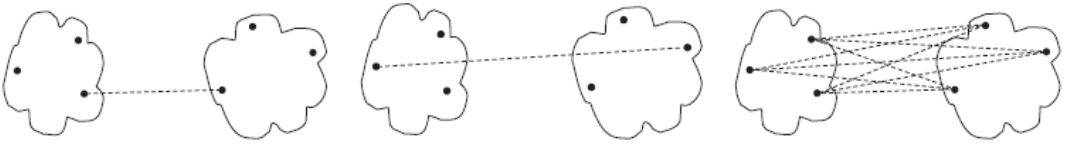
\includegraphics[width=\textwidth]{pics/minmax.png}
			\caption{Min, Max and group average}
		\end{figure}

		\clearpage
		\subsection{Specific Techniques}

		In this section we will go through an example of single and complete link with 
		data points. In the figure below, we see the example data of six points with x and y 
		positions and the distance from each point to all other points. We always start with 
		getting two clusters with 2 points in each that have the smallest distance, then 
		we start merging with MIN or MAX linking.
			
			\begin{figure}[H]
				\centering
				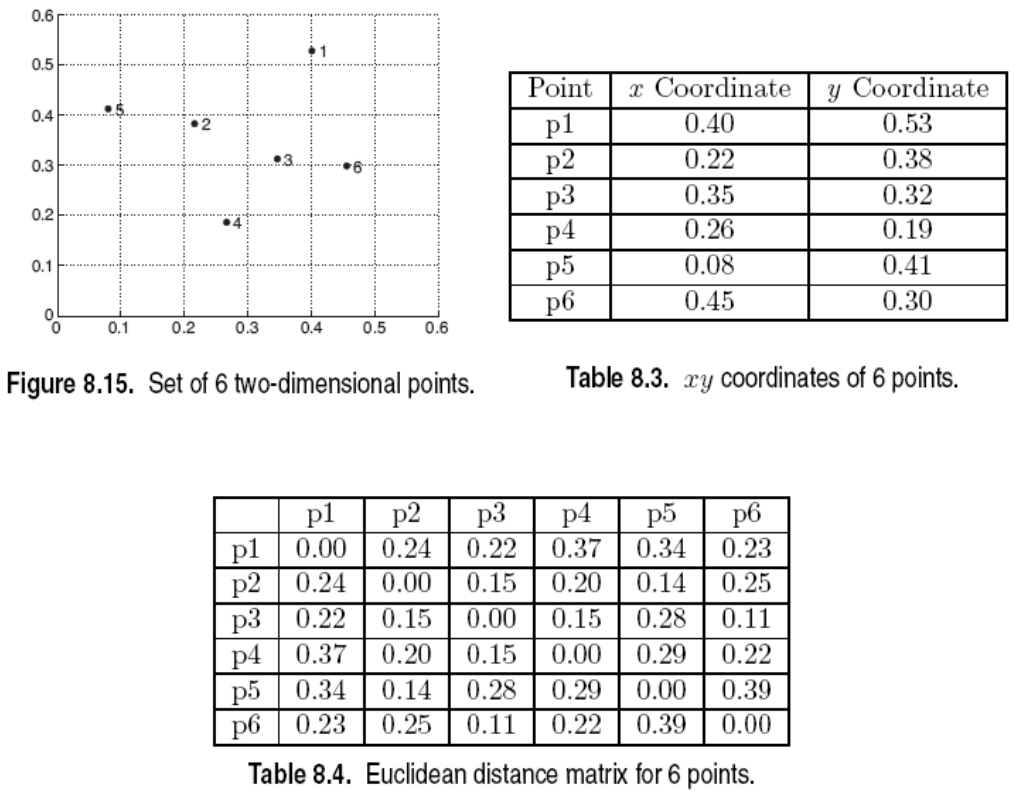
\includegraphics[scale=0.28]{pics/datapoints.png}
			\end{figure}

		{\bf Single Link (MIN):} for the single link or MIN version of hierarchical clustering, 
		the proximity of two clusters is defined as a minimum of the distance (maximum of the 
		similarity) between any points in the two different clusters. Using graph terminology, 
		if you start with all points as singleton clusters and add link between points one at 
		a time, shortest links first, then these single links combine the points into clusters. 
		The figure below shows the result of applying the single link technique to our example
		data set of six points.

		We see that the distance between point 3 and 6 is 0.11, and that is the height at which they
		are joined into one clusterin the dendrogram. As another example, the distance between
		clusters \{3,6\} and \{2,5\} is given by:

		{\color{red} $dist(\{3,6\}, \{2,5\})$ = min(dist(3,2), dist(6.2), dist(3,5), dist(6,5))
		= min(0.15, 0.25, 0.28, 0.39) = 0.15}


			\begin{figure}[H]
				\centering
				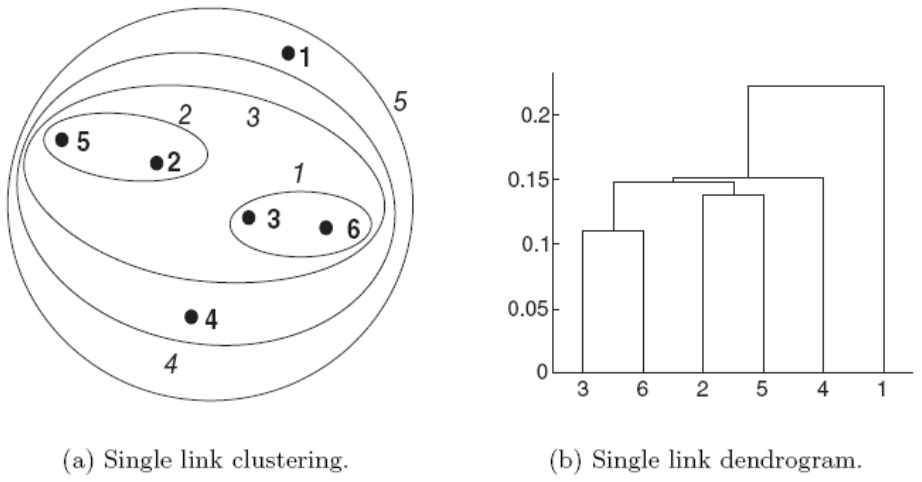
\includegraphics[scale=0.3]{pics/minlink.png}
				\caption{Results from the single link}
			\end{figure}			
		\clearpage
		{\bf Complete Link (MAX/CLIQUE):} For the complete link version of the  hierarchical clustering,
		the proximity of two clusters is defined as the maximum of the distance  (minimum of the 
		similarity) between any two points in the two different clusters. Using graph terminology,
		if you start with all points as singleton clusters and add links between points one at a time,
		shortests links first, then a group of points is not a cluster until all points in it are 
		completely linked, i.e., form a clique. 
		\{3,6\} and \{5,2\} is the two first clusters. We know need to merge with a new point or cluster:

		{\color{red} dist(\{3,6\}, \{4\}) = max(dist(3,4), dist(6,4)) = max(0.15, 0.22) = 0.22}

		{\color{blue} dist(\{3,6\}, \{2,5\}) = max(dist(3,2), dist(6,2), dist(3,5), dist(6,5)) = 
		max(0.15, 0.25, 0.28, 0.39)	= 0.39}

		{\color{orange} dist(\{3,6\}, \{1\}) = max(dist(3,1), dist(6,1)) = max(0.22, 0.23) = 0.23}

		We can see that merging cluster \{3, 6\} with \{4\} gives the minimum distance. It is
		very confusing using both terms min and max!

			\begin{figure}[H]
				\centering
				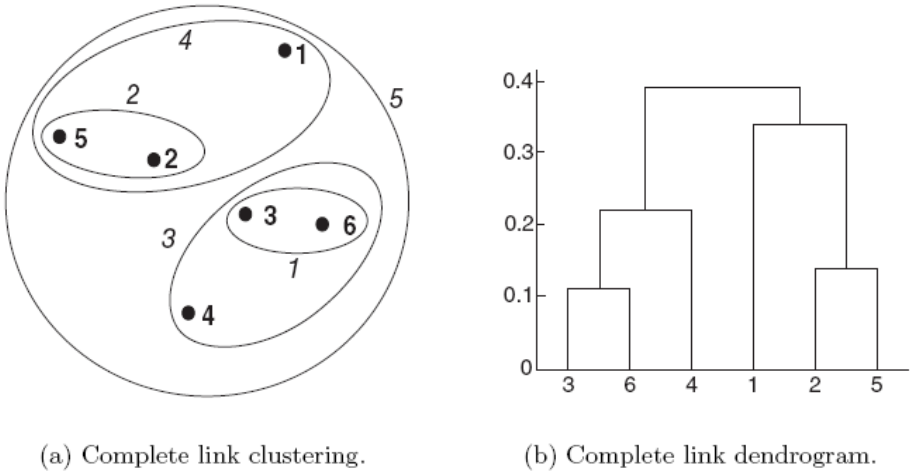
\includegraphics[scale=0.3]{pics/completelink.png}
				\caption{Results from the complete link}
			\end{figure}

		\clearpage
		{\bf Group Average:} For the group average version of hierarchical clustering, the
		proximity of two clusters is defined as the average pairwise proximity among all pairs of
		points in the different clusters. This is an intermediate approach between the single
		and complete link appraches. Thus, for group average, the cluster proximity 
		$proximity(C_{i}, C_{j})$ of clusters $C_{i}$ and $C_{j}$, which are of size $m_{i}$
		and $m_{j}$, respectively, is expressed by the following equation:

		\begin{equation}
			proximity(C_{i}, C_{j}) = \frac{\sum_{x \in C_{j}, y \in C_{j}} proximity(x,y)}{m_{i}*m_{j}}
		\end{equation}

		Here are some calculations from the 4'th iteration:

		{\color{red} dist(\{3, 6, 4\}, \{1\}) = (0.22 + 0.37 + 0.23) / (3*1) = 0.28}

		{\color{blue} dist(\{2, 5\}, \{1\}) = (0.2357 + 0.3421) / (2*1) = 0.2889}

		{\color{orange} dist(\{3, 6, 4\}, \{2, 5\}) = (0.15, 0.28, 0.25, 0.39, 0.2, 0.29) / (3*2) = 0.26}

		Here we choose to merge cluster \{3,6,4\} with cluster \{2,5\} because of the lowest
		proximity value. 


			\begin{figure}[H]
				\centering
				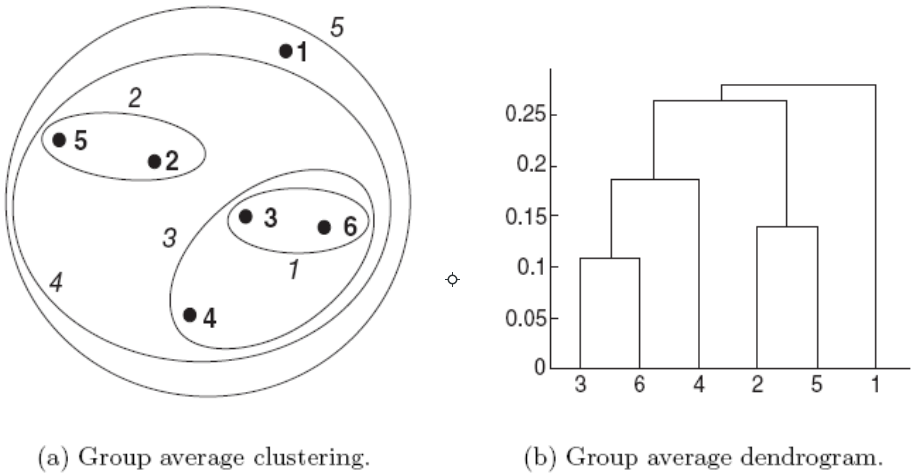
\includegraphics[scale=0.3]{pics/average.png}
				\caption{Results from the group average}
			\end{figure}

		{\bf Ward's method:} the proximity between two clusters is defined as the increase in 
		the squared error that results when two clusters are merged. This method uses the same
		objective function as k-means clustering. 
			
			\begin{figure}[H]
				\centering
				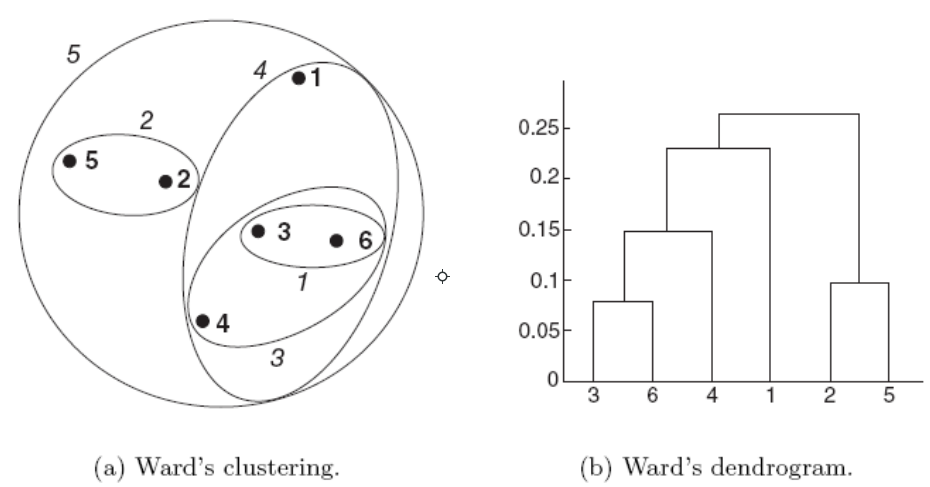
\includegraphics[scale=0.3]{pics/ward.png}
				\caption{Results from the Ward's method}
			\end{figure}
		\clearpage
		{\bf Strengths and weaknesses with hiaarchical clustering methods:}
			\begin{itemize}
				\item Single link (MIN)
					\begin{itemize}
						\item Fordel: Kan håndtere ikkeelliptiske former 
						\item Svakhet: Sensitiv til støy og outliers 
					\end{itemize}
				\item Complete link (MAX)
					\begin{itemize}
						\item Fordel: Mindre følsom for støy og outliers 
						\item Svakheter: Gir ofte oppdeling av store klynger,
						Tilbøyelighet mot kuleformet klynger, sensitiv til støy og outliers.
					\end{itemize}
				\item Group Average:
					\begin{itemize}
						\item Kompromiss mellom MIN og MAX 
						\item Styrke: Mindre følsom for støy og outliers 
						\item Svakhet: Tilbøyelighet mot kuleformet klynger
						\item Problem: dyrt å utregne
					\end{itemize}
			\end{itemize}

	\section{DBSCAN}		

		Density-based clustering locates regions of high density that are seperated
		from one another by regions of low density. DBSCAN is a simple and effective
		density-based clustering algorithm. 

		\subsection{Traditional Density: Center-Based Approach}

		{\bf Classification of points according to center-based density:}
		\begin{itemize}
			\item {\bf Core points:} in the enterior of a dense region (a core point).
			A point is a core point if the number of points within a given neigborhood around the 
			point as determined by the distance function and a user specified distance 
			parameter, {\it Eps}, exceeds a certain threshold, {\it MinPts}, which is also a
			user-specified parameter.  
			\item {\bf Border points:} on the edge of a dense region (a border point).
			\item {\bf Noise points:} in a sparsely occupied region (a noise or background point).
		\end{itemize}


			\begin{figure}[H]
				\centering
				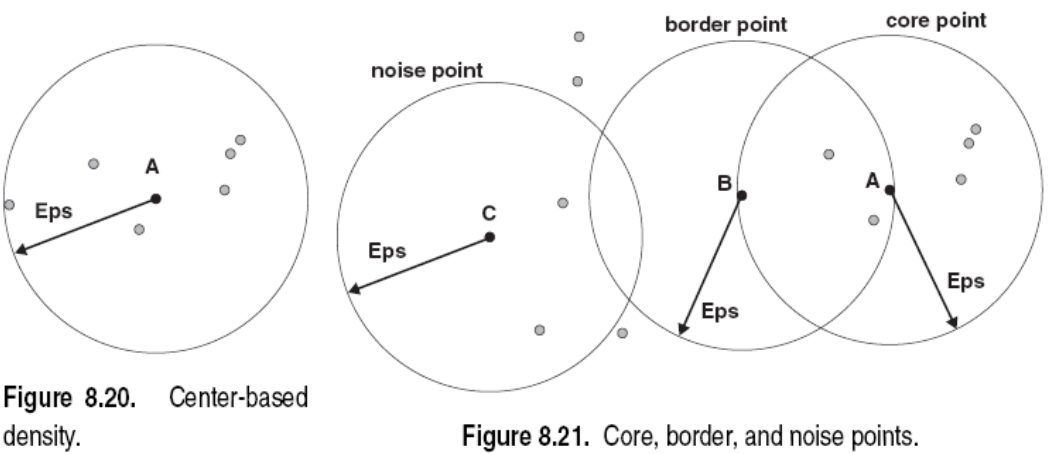
\includegraphics[width=\textwidth]{pics/dbscan.png}
			\end{figure}

		\subsection{DBSCAN Algorithm}

			The DBSCAN can be informally described as follows. Any two core points
			that are close enough - within a distance {\it Eps} of ine another - 
			are put in the same cluster. Likewise, any border point that is close 
			enough to a core point is put in the same cluster as the core point.
			(Ties may need to be resolved if a border point is close to core points
			from different clusters.) Noise points are discarded. 

			\begin{enumerate}
				\item Label all points as core, border, or noise points.
				\item Eliminate noise points
				\item Put an edge between all core points that are within {\it Eps} of each other
				\item Make each group of connected core points into a separate cluster
				\item Assign each border point to one of the clusters of its associated core points.
			\end{enumerate}

			\begin{figure}[H]
				\centering
				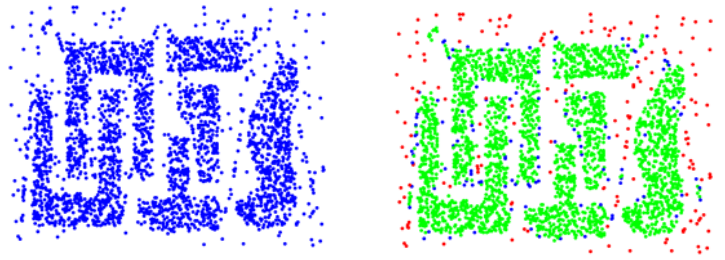
\includegraphics[scale=0.5]{pics/dbscan2.png}
				\caption{1) Original data points, 2) {\color{green}core points}, {\color{blue}border points}, and
				{\color{red}noise points}.}
			\end{figure}

			{\bf Strengths and Weaknesses}
				\begin{itemize}
					\item {\bf Fungerer når:} Motstandsdyktig mot støy og kan håndtere klynger med forskjellige former 
					og størrelse
					\item {\bf Fungerer ikke når:} Varierende tetthet, Høydimensjonale data.
					\item Er sensitiv i forhold til valg av eps og MinPts.
					\item Cluster som ligger inne i støy fungerer ikke så bra. 
				\end{itemize}

	\clearpage
	\section{Cluster Evaluation}

		In supervised classification, the evaluation of the resulting classification model
		is an integral part of the proces of developing a classification model, and
		there are well-accepted evaluation measures and procedures, e.g., accuracy
		and cross-validation, respectively. However, because of its very nature, cluster
		evaluation is not a well-developed or commonly used part of cluster analysis.

		There are a number of different clusters - in some sense, each clustering 
		algorithm defines its own type of clusters - it may seem that each situation 
		might require a different evaluation measure. Here are a clustering example with
		different algorithms used:

		\begin{figure}[H]
			\centering
			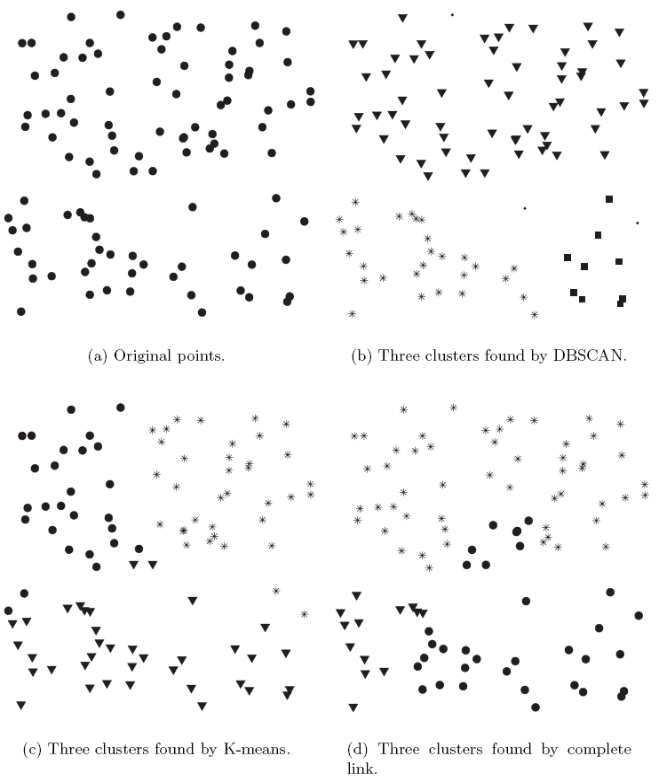
\includegraphics[scale=0.4]{pics/threeclusters.png}
		\end{figure}

		{\bf Important issues for cluster validation:}
		\begin{enumerate}
			\item Determining the cluster tendency of a set of data, i.e., distinguishing
			between wheter non-random structure actually exists in the data.
			\item Determining the correct number of clusters
			\item Evaluating how well the results of a cluster analysis fit the data
			without reference to external information.
			\item Comparing the results of a cluster analysis to externally known results,
			such as externally provided class labels.
			\item Comparing two sets of clusters to determine which is better. 
		\end{enumerate}

		\clearpage
		Evaluation measures, or indices, that are applied to judge various aspects of cluster validity
		are traditionally classified into the following three types:

			\begin{itemize}
				\item {\bf Unsupervised:} measure the goodness of a clustering structure without
				respect to external information. An example of this is SSE. 
				Unsupervised measures of cluster validity are often further divided into
				two classes: measures of {\bf cluster cohesion} (compactness, tightness), which
				determine how closely related the objects in a cluster are, and measures
				of {\bf cluster separation} (isolation), which determine how distinct or well
				separated a cluster is from other clusters. Unsupervised measures are often
				called {\bf internal indices} because they use only information present in the
				data set.
				\item {\bf Supervised:} measures the extent to which the clustering structure
				discovered by a clustering algorithm matches some external structure. 
				An example of supervised index is entropy, which measures how well a cluster
				labels match externally supplied class labels. Supervised measures are 
				often called {\bf external indices} becuase they use information not present
				in the data set. 
				\item {\bf Relative:} Compares different clustering or clusters. A relative 
				cluster evaluation measure is supervised or unsupervised evaluation measure 
				that is used for the purpose of comparison. As an example, two K-means clusterings
				can be compared using either the SSE or entropy. 
			\end{itemize}

		\subsection{Unsupervised Cluster Evaluation Using Cohesion and Sparation}
			In general, we can consider expressing overall cluster validity for a set of 
			K clusters as a weighted sum of the validity of individually clusters:

				\begin{equation}
					overall Validity = \sum_{i=1}^{K} w_{i} validity(C_{i})
				\end{equation}

			The validity function can be cohesion, spearation, or some combination of 
			these quantities.

			{\bf Graph-based view of Cohesion and separation}

			For graph-based clusters, the cohesion of a cluster can be defined as the sum
			of the weights of the links in the proximity graph that connect points whitin 
			the cluster. 
			Likewise, the separation between two clusters can be measured by the sum of
			weights of the links from points in one cluster to point in the other cluster.
			The proximity function can be a similarity, a dissimilarity, or a simple function
			of these quantities. 

				\begin{equation}
					cohesion(C_{i}) = \sum_{x \in C_{i}, y \in C_{i}} proximity(x,y)
				\end{equation} 

				\begin{equation}
					separation(C_{i}, C_{j}) = \sum_{x \in C_{i}, y \in C_{j}} proximity(x,y)
				\end{equation} 

			\begin{figure}[H]
				\centering
				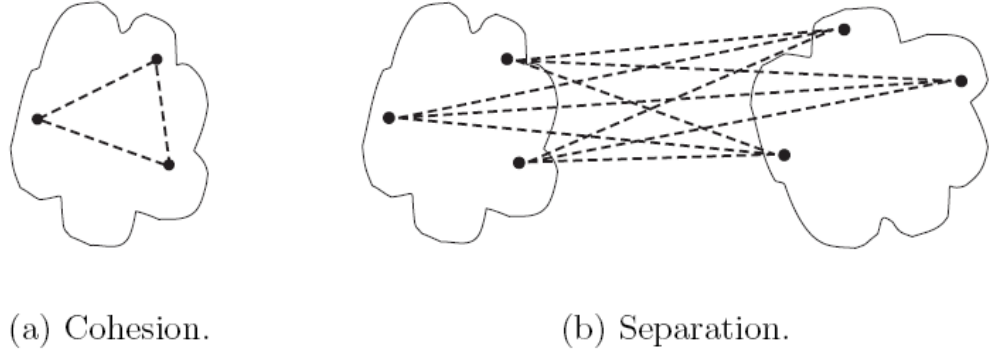
\includegraphics[scale=0.3]{pics/graphbased.png}
			\end{figure}


			{\bf Prototype-based View of Cohesion and Separation}

			For prototype-based clusters, the cohesion of a cluster can be defined as the sum
			of proximties with respect to the prototype (centroid or mendoid) of the cluster.

			\begin{equation}
				cohesion(C_{i}) = \sum_{x \in C_{i}} proximity(x, c_{i})
			\end{equation}

			\begin{equation}
				separation(C_{i}, C_{j}) = proximity(c_{i}, c_{j})
			\end{equation}

			\begin{equation}
				separation(C_{i}) = proximity(c_{i}, c)
			\end{equation}

			$c_{i}$ is the prototype (centroid) of cluster $C_{i}$, and c is the overall
			prototype (centroid). 

			\begin{figure}[H]
				\centering
				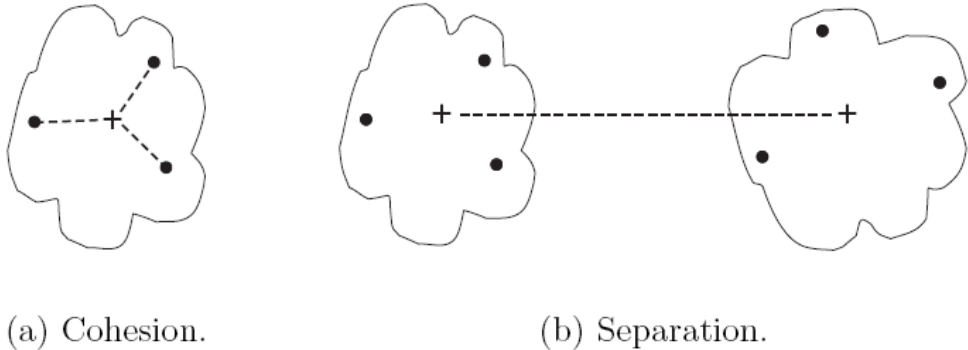
\includegraphics[scale=0.3]{pics/prototypebased.png}
			\end{figure}

			{\bf Evaluating Individual Clusters and Objects}

				So far, we have focused on using cohesion and separation in the overall
				evaluation of a group of clusters. Many of these measures of cluster
				validity also can be used to evaluate individual clusters and objects.

				A cluster that has a high value of cohesion may be considered better than
				a cluster that has a lower value. This information often can be used to 
				improve the quality of a clustering. If for example, a cluster is not
				very cohesive, then we may want to split it into serveral subclusters. 
				On the other hand, if two clusters are relatively cohesive, ut not
				well separated, we may want to merge them into a single cluster. 

				We can also evaluate the objects within a cluster in terms of their
				contribution to the overall cohesion or separation of the cluster. 
				Objects that contribute more to the cohesion and separation are near the 
				"interior" of the cluster. Those objects for which the opposite is true
				are probably near the "edge" of the cluster. 

				{\bf The Silhouette Coefficient:}

				The popular method of silhouette coefficients combines both cohesion and
				separation. The following steps explain how to compute the silhouette coefficient
				for an individual point., a process that consists of the following three steps.
				We use distances, but an analogous approach can be used for similarities.

				\begin{enumerate}
					\item For the $i^{th}$ object, calculate its average distance to all other
					objects in its cluster. Call this value $a_{i}$.
					\item For the $i^{th}$ object annd any cluster not containing the object,
					calculate the object's average distance to all the objects in the given
					cluster. Find the minimum such value with respect to all clusters; call
					this value $b_{i}$.
					\item For the $i^{th}$ object, the silhouette coefficient is 
					$s_{i} = (b_{i} - a_{i})/max(a_{i},b_{i})$.
				\end{enumerate}

				The value of the silhouette can vary between -1 and 1. A negative value is
				undesirable because this corresponds to a case in which $a_{i}$, the average
				distance to points in the cluster, is greater than $b_{i}$, the minimum
				average distance to points in another cluster. We want the silhouette
				coefficient to be positive, and for $a_{i}$ to be as close to 0 as possible,
				since the coefficient assumes its maximum value of 1 when $a_{i}$ = 0.

				We can compute the average silhouette coefficient of a cluster by simply
				taking the average of the shilouette coefficients of points belonging to the
				cluster. An overall measure of the goodness of a clustering can be obtained
				by computing the average silhouette coefficient of all points. 


		\subsection{Unsupervised Cluster Evaluation Using the Proximity Matrix}

			In this section, we examine a couple of unsupervised approaches for assessing
			cluster validity that are based on the proximity matrix. 

			{\bf Measuring Cluster Vality via Correlation}

			If we are given the similarity matrix for a data set and the cluster labels from
			a cluster analysis of the data set, then we can evaluate the goodness of the 
			clustering by looking at the correlation between {\bf actual similarity matrix} and an 
			{\bf ideal version of the similarity matrix} based on the cluster labels. 

			More Specifically, an ideal cluster is one whose points have a similarity
			of 1 to all points in the cluster, and a similarity of 0 to all points
			in other clusters.

			The {\bf ideal similarity matrix} is constructed by creating a matrix that has one
			row and one column  for each data point, and assigning a 1 to an entry if the 
			associated pair of points belongs to the same cluster. All other entries are 0.
			High correlation between the ideal and actual simularity matrices indicates
			that the points that belong to the same cluster are close to each other, while
			low correlation indicates the opposite. 
			Since the actual and ideal similarity matrices are symmetric, the correlation is
			calculated only among the n(n-1)/2 entries below or above the diagonal of the matrices.


		\subsection{Internal goals: Cohesion and seperation}

			\begin{figure}[H]
				\centering
				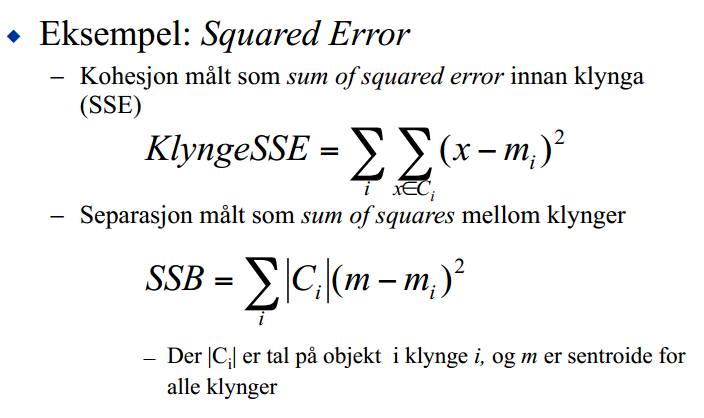
\includegraphics[scale=0.5]{pics/cosep.png}
			\end{figure}
			\begin{figure}[H]
				\centering
				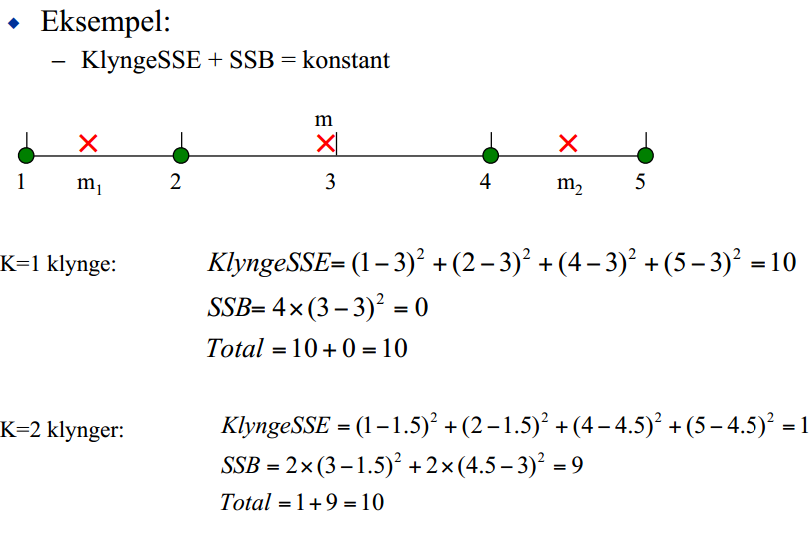
\includegraphics[scale=0.5]{pics/cosep2.png}
			\end{figure}

		\subsection{Internal goals: ENtropy and Purity}

		\begin{figure}[H]
				\centering
				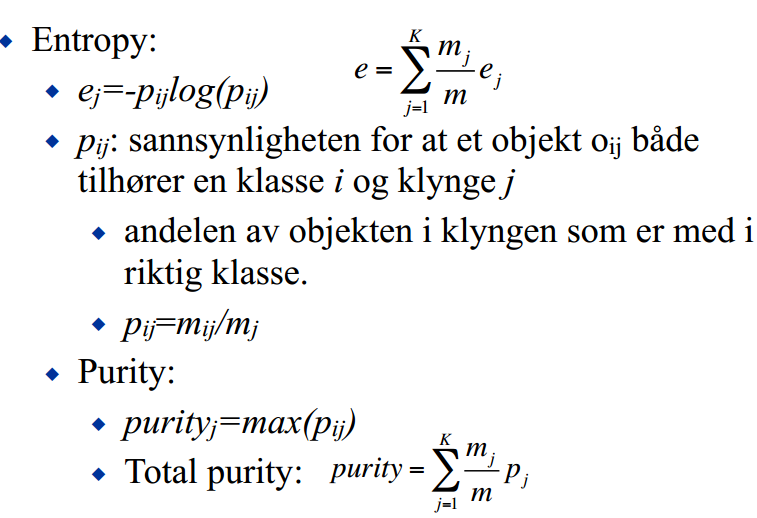
\includegraphics[scale=0.5]{pics/entpu.png}
			\end{figure}


